\chapter{Introduction}
\label{ch1}

Behind the great success of medical imaging, a crisis is looming: the number of imaging studies, the workload of radiologists, and the health care cost related to imaging are rising rapidly. 
We are facing an unprecedented challenge: image data explosion---modern imaging systems generate enormous volumes of data, far exceeding human abilities for interpretation. 
What is critical, however, is not the images themselves, but rather the clinically relevant information contained within them. To automatically glean this information from medical images, deep learning holds great promise~\citep{goodfellow2016deep} in improving diagnosis accuracy and efficiency. 

Modern computer-aided diagnosis has greatly benefited from deep learning advances in disease/organ detection, classification, and segmentation. There is no doubt that the impact of deep learning will be phenomenal---most medical images will be interpreted by computers even before they reach a radiologist in the future. Many studies have demonstrated promising results in complex diagnostics spanning dermatology~\citep{esteva2017dermatologist,haenssle2018man}, radiology~\citep{cheng2016computer,cicero2017training,kooi2017large,ardila2019end}, ophthalmology~\citep{gulshan2016development,poplin2018prediction,de2018clinically}, and pathology~\citep{beck2011systematic,cirecsan2013mitosis,charoentong2017pan,yamamoto2019automated}, to name a few. However, developing such systems is impeded by a significant barrier: deep learning is data hungry by nature, demanding large-scale, high-quality annotated datasets; otherwise, deep learning often results in algorithms that perform poorly and lack generalizability on new data.


%%%%%%%%%%%%%%%%%%%%%%%%%%%%%%%%%%%%%%%%%%%%
\begin{figure}[t]
%\footnotesize
\begin{center}
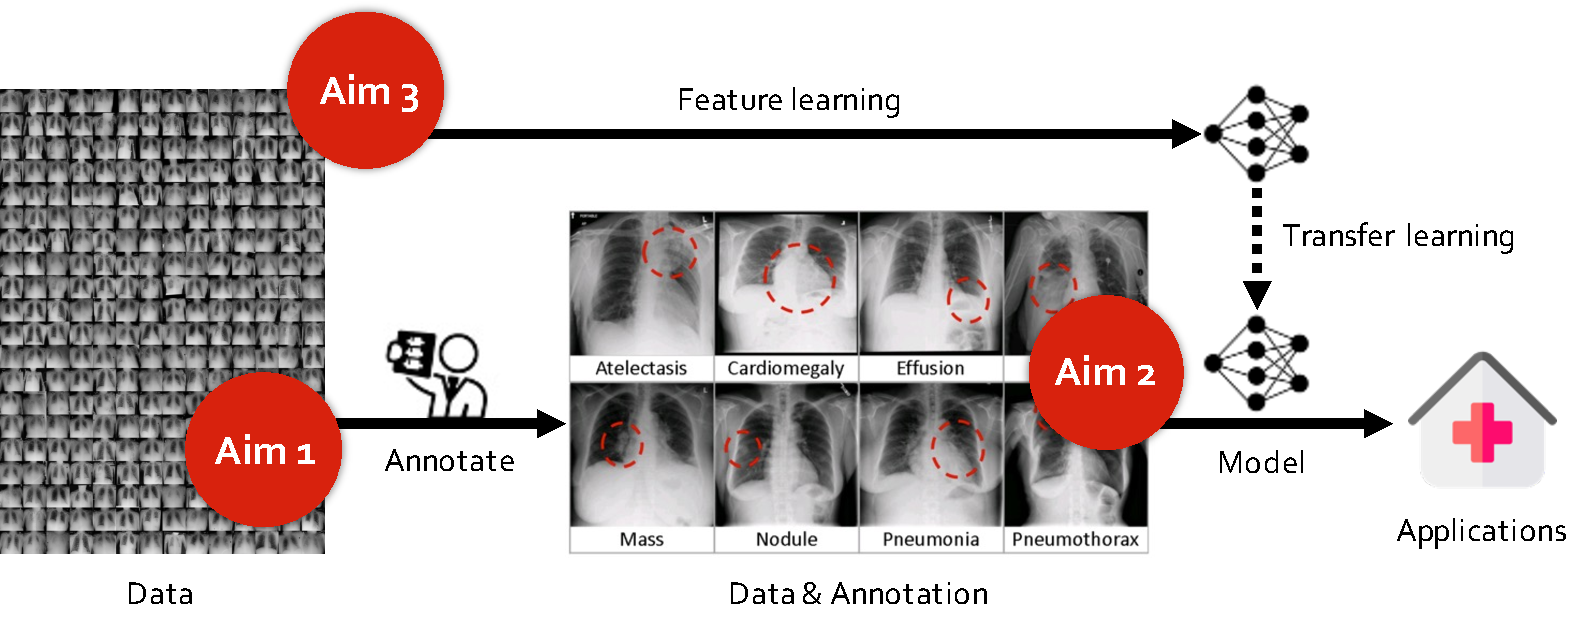
\includegraphics[width=1.0\linewidth]{Figures/CH1/fig_hypothesis.pdf}
\end{center}
\caption[Outline of the Dissertation]
{The overall pipeline of deep learning algorithms engaged in healthcare process: (1) obtaining annotation from human expert; (2) training and validating a deep model using these annotation; and (3) deploying the deep model in clinical practice. Our objective is to minimize manual annotation efforts for rapid, precise computer-aided diagnosis systems. In doing so, we have outlined three specific aims: (1) acquiring necessary annotation efficiently from human experts; (2) utilizing existing annotation effectively from advanced architecture; and (3) extracting generic knowledge directly from unannotated images. As a result, given the same amount of annotation, our deep learning models can yield higher performance; maintaining the similar performance, we ask for less annotation.}
\label{ch1:fig:hypothesis}
\end{figure}
%%%%%%%%%%%%%%%%%%%%%%%%%%%%%%%%%%%%%%%%%%%%


Annotating medical images is not only tedious and time consuming, but it also requires costly, specialty-oriented knowledge and skills, which are not easily accessible. To overcome this barrier, our objective is to develop innovative, annotation-efficient methodologies by exploiting the intrinsic characteristics of medical images. In this dissertation, we seek to address the critical problem: \textit{How to develop efficient and effective deep learning methods for medical applications where large annotated datasets are unavailable}.
The dream of ``big data'' induces the misconception that more data can promise higher performance, so we keep asking human experts to annotate as many data as possible. However, the performance of deep models is not linearly correlated to the number of annotated data; instead, there comes the plateau where even annotating more data cannot further improve the accuracy. This is due to the inevitable human error in annotation. Every task and model will encounter this bottleneck plateau. In essence, the amount of annotated data that can lead to the performance plateau is dependent on the complexity of the task, but it is also exceedingly influenced by the efficacy of the learning strategy and the capacity of the model architecture. This dissertation mainly focuses on optimizing the learning strategy and maximizing the model capacity, leading to our hypothesis that:

\bigskip\bigskip
\begin{tcolorbox}
With a small part of the dataset annotated, we can deliver deep models that match, or even outperform those that require annotating the entire dataset.
\end{tcolorbox}


We base this hypothesis on three pillars as outlined in~\figurename~\ref{ch1:fig:hypothesis}. First, wisely selecting important samples can reduce the annotation cost in comparison with random selection. A common procedure of determining which sample needs to be annotated first by human experts is called ``human-in-the-loop'' active learning. Second, multi-scale feature aggregation in deep models can address tasks with higher complexity. Image segmentation, as an example, is one of the most complicated tasks in medical image analysis, demanding rich image features that span levels from low to high, and scales from small to large. Finally, deep models with general-purpose image representation can be built upon the consistent, recurrent anatomical structure embedded in medical images. We envision that these generic models can serve as a primary source of transfer learning for many medical imaging tasks, even with limited annotated data. 


%%%%%%%%%%%%%%%%%%%%%%%%%%%%%%%%%%%%%%%%%%%%
\begin{figure}[t]
%\footnotesize
\begin{center}
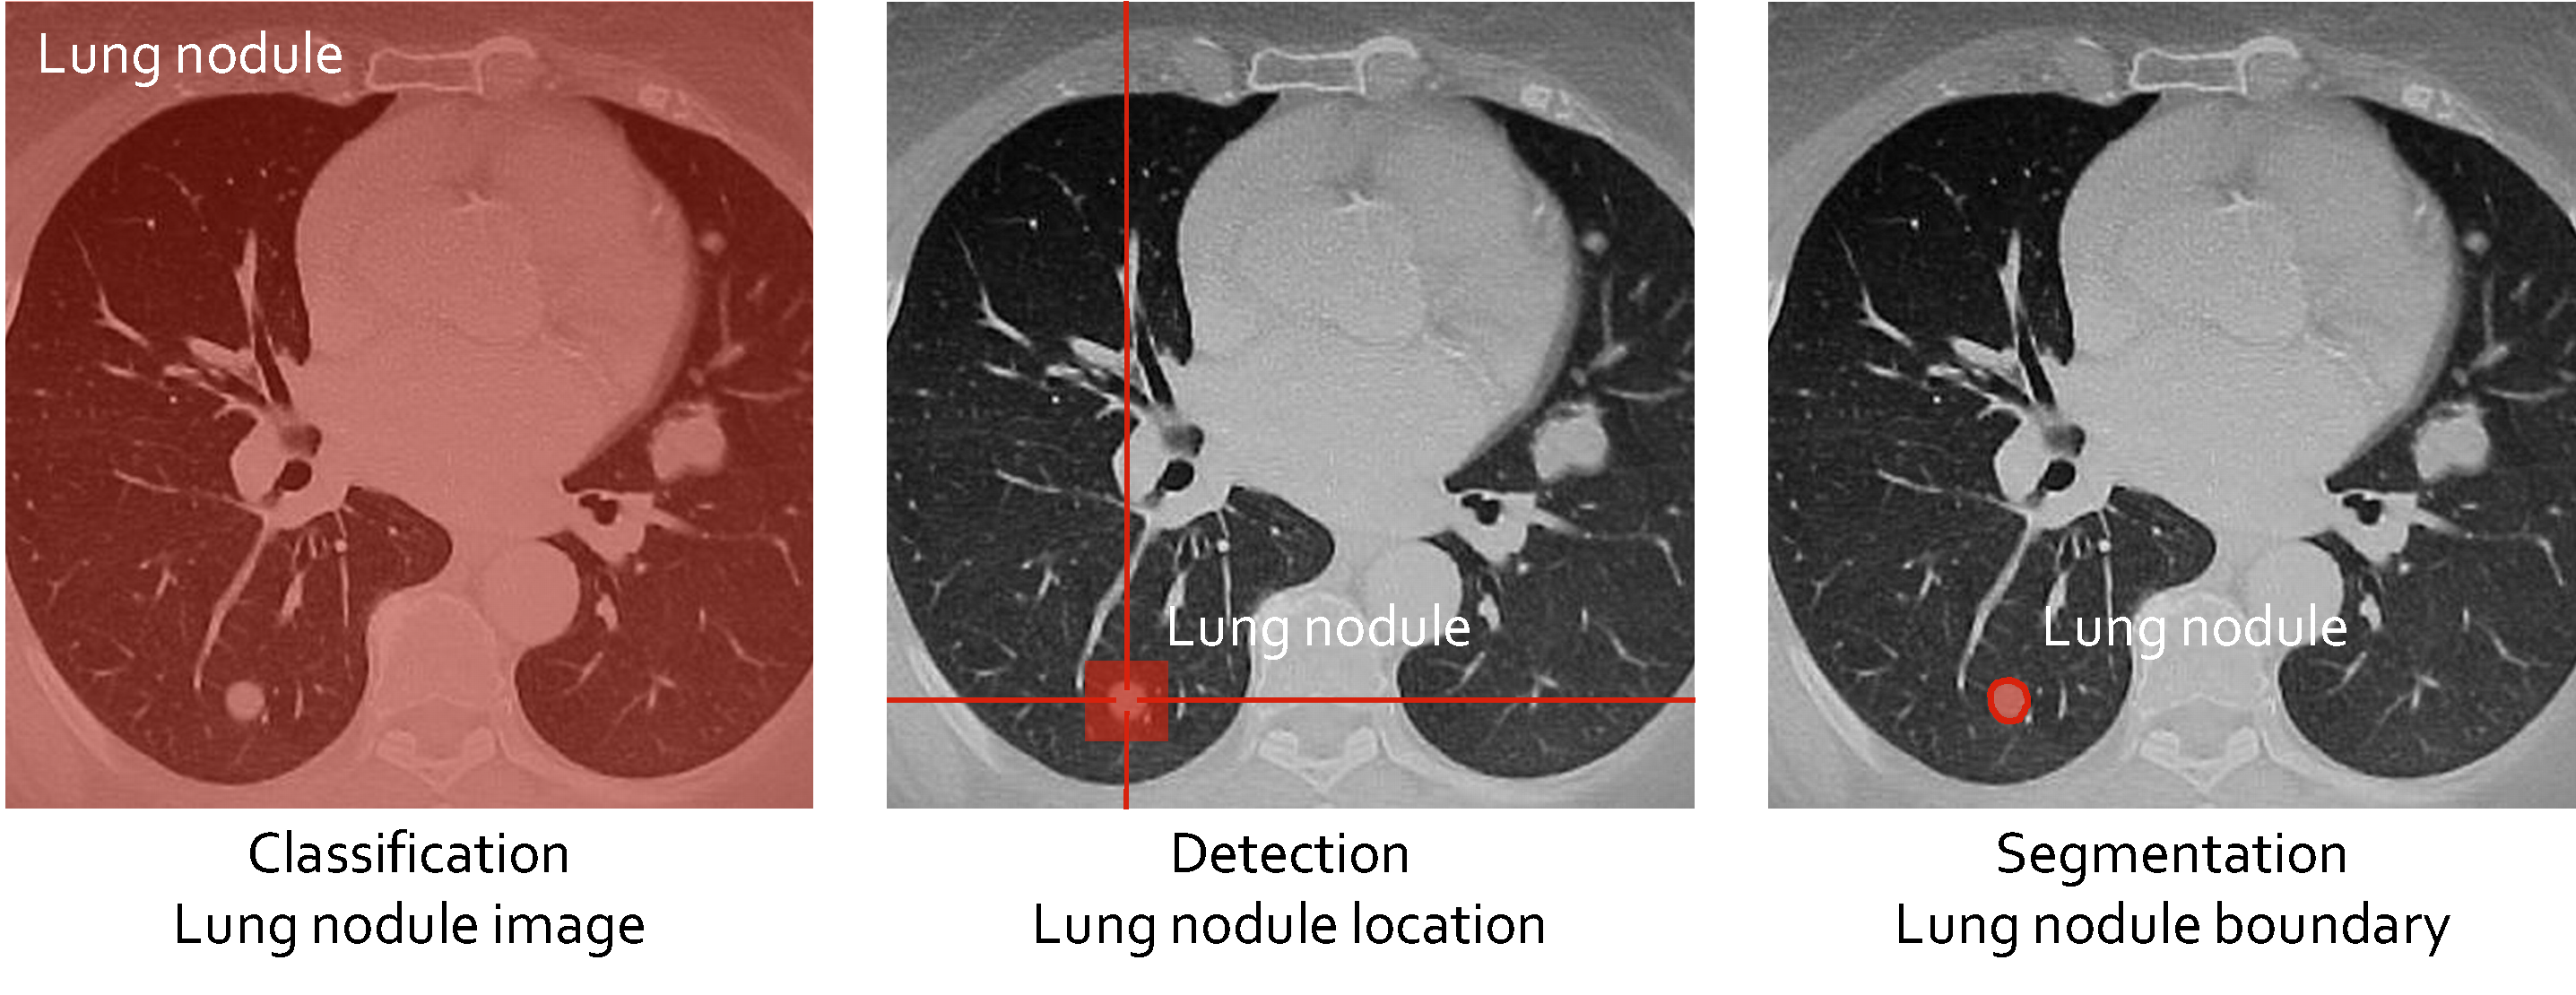
\includegraphics[width=1.0\linewidth]{Figures/CH1/fig_annotation_types.pdf}
\end{center}
\caption[What Is Annotation?]{
When harnessing large-scaled annotated datasets to advance medical imaging, the key question is \textit{what annotation should be collected}. There are several types of annotation as per the task requirements in clinical practice. Different types of annotation come with different associated costs. 
For example, to annotate lung nodules for the tasks of classification, detection, and segmentation, human experts must consider different types of annotation---labeling the existence of the nodule, indicating its location, and drawing a contour of its boundary, respectively. 
These three types of annotation are anticipated to span manual annotation efforts from easy to hard, annotation qualities from coarse to fine, and annotation time from short to long.}
\label{ch1:fig:annotation_types}
\end{figure}
%%%%%%%%%%%%%%%%%%%%%%%%%%%%%%%%%%%%%%%%%%%%


\section{What is Annotation?}
\label{ch1:challenge_opportunity:annotation}


Annotation is the process of assigning labels to raw data in preparation for training the computer on the pairs of data and labels; then, the computer can predict labels for many new data. For the development of deep learning methods, supervised learning is the most prominent learning paradigm, in which the annotation is used to guide model learning and error propagating. Therefore, annotating datasets is an indispensable stage of data processing in the AI era. For natural imaging, data is collected from numerous photos from social media and annotation is often given by non-experts through crowdsourcing~\citep{kovashka2016crowdsourcing}. Annotating medical images, however, demands costly, specialty-oriented knowledge and skills, which are not easily accessible. Thereby, medical image annotation is done mainly by human experts, who manually and precisely annotate the existence, appearance, and severity of diseases in each medical image with the help of appropriate software tools, such as Lionbridge AI, ITK-SNAP, Cogito, Labelbox, 3D Slicer, etc. For some abnormalities that experts cannot immediately recognize from images, biopsy outcomes can also be used as annotation. \figurename~\ref{ch1:fig:annotation_types} illustrates different types of annotation in medical imaging. This dissertation utilizes the annotation tagged with existing benchmark datasets as the gold standard to train and validate deep learning methods.



\section{The Barrier: Not Enough Annotation}
\label{ch1:challenge_opportunity:barrier}

Deep learning methods are data hungry by nature, requiring sufficiently large-scale, high-quality, well-integrated annotated datasets---more so than other algorithms. Recent studies suggest that, to match human diagnostic precision, deep learning methods require 42,290 radiologist-annotated CT images for lung cancer diagnosis~\citep{ardila2019end}, 137,291 radiologist-annotated mammograms images for breast cancer identification~\citep{mckinney2020international}, 129,450 dermatologist-annotated images for skin cancer classification~\citep{esteva2017dermatologist}, and 128,175 ophthalmologist-annotated retinal images for diabetic retinopathy detection~\citep{gulshan2016development}. Without such large annotated datasets, deep learning often results in algorithms that perform poorly and lack generalizability on new data. Nonetheless, rarely do we have a perfectly-sized and carefully-annotated dataset to train, validate, and test a deep learning model, particularly for applications in medical imaging, where both data and annotation are expensive to acquire. This requirement becomes more challenging in situations when quickly responding to global pandemics or when scaling up to several rare diseases where it is impractical to collect large quantities of annotated data. Manual annotation of medical images is still the key bottleneck in translating deep learning advancements into clinically useful computer-aided diagnosis (CAD) systems. Consequently, there is a pressing need for innovative methodologies that enable annotation-efficient deep learning for medical image analysis.






%In the following section, we extensively review the frontiers in technology that tackle the significant barrier of annotation acquisition by harnessing the three unique advantages, while demonstrating the novelty of the methodologies that we have developed.


\section{Overview of Contributions}
\label{ch1:thesis_outline}

This dissertation starts with a brief introduction of the concept of ``annotation'', followed by the motivation of developing annotation-efficient deep learning for computer-aided diagnosis. Specifically, we describe some of the greatest achievements of deep learning in medical imaging, associated with the number of annotation efforts behind these successes, underlining the desire to improve the efficiency of their development procedure. 


Chapter~\ref{ch2} compiles the role of annotation in developing computer vision algorithms from a historical perspective, shedding light on a discussion of current limitations and future premises. We then outline three unique advantages that have been stimulating the development of annotation-efficient deep learning for computer-aided diagnosis, including continual learning capabilities, representation learning capabilities, and recurrent anatomical structures. This chapter closes with an extensive review of how technical advancements address the barrier of annotation sparsity by harnessing the three unique advantages. Along the way, we highlight the novelty of the methodologies that we have developed by contrasting them with existing approaches. 


    
Chapter~\ref{ch3} discusses how to actively select patients/samples for annotation. We have devised a novel annotation query procedure to naturally integrate active learning and transfer learning into a single framework, reducing the manual annotation cost by at least half. Specifically, we combine newly annotated data with misclassified data by the current model, supplemented with continuous fine-tuning to accelerate model training, thereby encouraging the reuse of data. This procedure begins with a completely empty annotated dataset, improving the deep model's performance by actively selecting the most informative and representative samples. Studying different active learning strategies is important because an efficient ``human-in-the-loop'' procedure encourages label and model reuse, while additionally assisting radiologists in quickly dismissing patients with negative results. This work was one of only five papers in biomedical imaging accepted by CVPR-2017~\citep{zhou2017fine}. Consequently, this technique has been presented in several journal publications~\citep{zhou2019integrating,zhou2021active} and filed as a US patent application.
    
Chapter~\ref{ch4} discusses how to design advanced architectures that achieve annotation efficiency. We have designed an advanced neural architecture, named UNet++, for disease and organ segmentation, leveraging the power of existing annotation for improved performance. In doing so, we employed an efficient ensemble of U-Nets~\citep{falk2019u} of varying depths, which partially share an encoder and co-learn simultaneously using deep supervision, to alleviate the unknown network depth. 
We also redesigned skip connections to accommodate feature aggregation of varying semantic scales in decoder sub-networks. 
Finally, we devised a pruning scheme to accelerate model inference speed, allowing CAD systems to accomplish automatic disease detection using the ordinary desktop/laptop PCs commonly employed in clinical practice. This algorithmic innovation is significant because the learning capability of a deep model relies heavily on the use of multiple feature aggregation that can automatically learn representations from the data. UNet++ has been quickly adopted by the research community, listed among the most popular articles in IEEE TMI since published~\citep{zhou2018unet++,zhou2019unet++}; more recently, UNet++ has been widely applied to segment lung infections caused by COVID-19~\citep{dong2020role,shi2020review}. 
    
Chapter~\ref{ch5} discusses how to learn generic knowledge from unannotated data. We have developed a framework that trains generic source models for medical imaging, enabling rapid progress and improved performance for various medical applications across numerous diseases, datasets, organs, and modalities. This framework exploits an advantage stemming from the consistent and recurrent anatomy intrinsic to medical images that has the unique potential to act as strong, yet free, supervision signals for deep models to learn robust image representation. The self-supervised representation learning is beneficial to the research community because generic pre-trained models can serve as a primary source of transfer learning for numerous medical imaging applications, leading to accelerated training and improved performance. This work received the MICCAI Young Scientist Award\footnote{\href{http://www.miccai.org/about-miccai/awards/young-scientist-award/}{http://www.miccai.org/about-miccai/awards/young-scientist-award/}}~\citep{zhou2019models} and was chosen as one of the selected contributions, receiving the MedIA Best Paper Award in Medical Image Analysis\footnote{\href{http://www.miccai.org/about-miccai/awards/medical-image-analysis-best-paper-award/}{http://www.miccai.org/about-miccai/awards/medical-image-analysis-best-paper-award/}}~\citep{zhou2021models}.

Chapter~\ref{ch6} discusses how our developed techniques impact the key facets of CAD systems. We first describe some of the most distinguished characteristics of medical images, which are the vital foundations and inspirations of the techniques presented in this dissertation. We then express the clinical needs and introduce imaging applications in healthcare. Moreover, we dive into the details of how our techniques improve performance and annotation efficiency in an exemplar CAD system for detecting pulmonary embolism from CTPA images. Our system achieves a sensitivity of 46\% at 2 false positives per scan, ranked third among the participating teams in the CAD-PE competition.
    
Chapter~\ref{ch7} concludes the dissertation with a discussion of the overall impact. 
% {\jlred Not only for medical applications, but also other visual applications, such as.}


Many people criticize that deep learning requires too much annotated data, while humans can learn from one or a few examples---this argument is biased. It is true that training computers to detect lung nodules, for example, from CTs requires tens of thousands of annotated images~\citep{ardila2019end}, while a college student can accomplish the same task after being exposed to a few examples from textbooks. Nevertheless, we would not expect an infant to detect lung nodules by only seeing this small number of examples. The capability of annotation-efficient human vision (the holy grail for the next generation of deep learning) is based on numerous everyday learning activities. It takes a village to develop such annotation-efficient deep learning, and the resulting algorithm may not be prepared for any of the specific visual tasks. Once done, however, the algorithm can be quickly adapted to numerous tasks by only asking for a small amount of annotation, like human vision. As the popular Chinese saying goes, \textit{sharpening the axe will not slow down the work of cutting wood}. Progress in this line of research can leverage the power of small annotated data to establish more effective deep learning methods, therefore, alleviating the time and cost for manually annotating a large amount of data and exerting computer-aided diagnosis for a wider range of disorders.

% Annotation-efficient deep learning is the dream of computer vision and medical imaging, as it can significantly reduce the overall human annotation efforts, promoting computer-aided diagnosis for a wider range of disorders.

% Progress in this line of research can establish effective deep learning methods by leveraging small annotated data, therefore, dramatically reducing manual annotation efforts and exerting computer-aided diagnosis for a greater range of disorders.